\section{Aufgabenstellung}
\label{sec:aufgabe}
Es soll ein Gerät entwickelt werden, das Bälle in einen Korb befördern kann.  
Das Spielfeld, auf dem die Aufgabe erledigt werden soll, ist dabei in 
\autoref{fig:playfield} dargestellt. Das Gerät befindet sich vor dem 
Startsignal im \mbox{\tikz{\draw[fill=yellow] (0,0) rectangle (0.25,0.25);} 
Startbereich} und darf die in \autoref{tab:device} definierten Abmessungen 
nicht überschreiten. Nach dem Startsignal darf sich der Roboter innerhalb von 
\mbox{\tikz{\draw[fill=yellow] (0,0) rectangle (0.25,0.25);} Start}- und 
\mbox{\tikz{\draw[fill=cyan] (0,0) rectangle (0.25,0.25);} Bewegungsbereich} 
bewegen. Der \mbox{\tikz{\draw[fill=red] (0,0) rectangle (0.25,0.25);} 
verbotene Bereich} darf jedoch weder berührt noch überragt werden. Im 
\mbox{\tikz{\draw[fill=green] (0,0) rectangle (0.25,0.25);} Zielbereich} 
befindet sich der Korb. Dieser wird erst direkt vor dem Startsignal platziert 
und muss vom Gerät  gefunden werden. Hinter dem Korb befindet sich eine Wand 
mit einer Höhe von 100 cm. Das Gerät muss die Aufgabe autonom absolvieren. 
\cite{hslu:aufgabe}
\begin{figure}[h!]
    \centering
    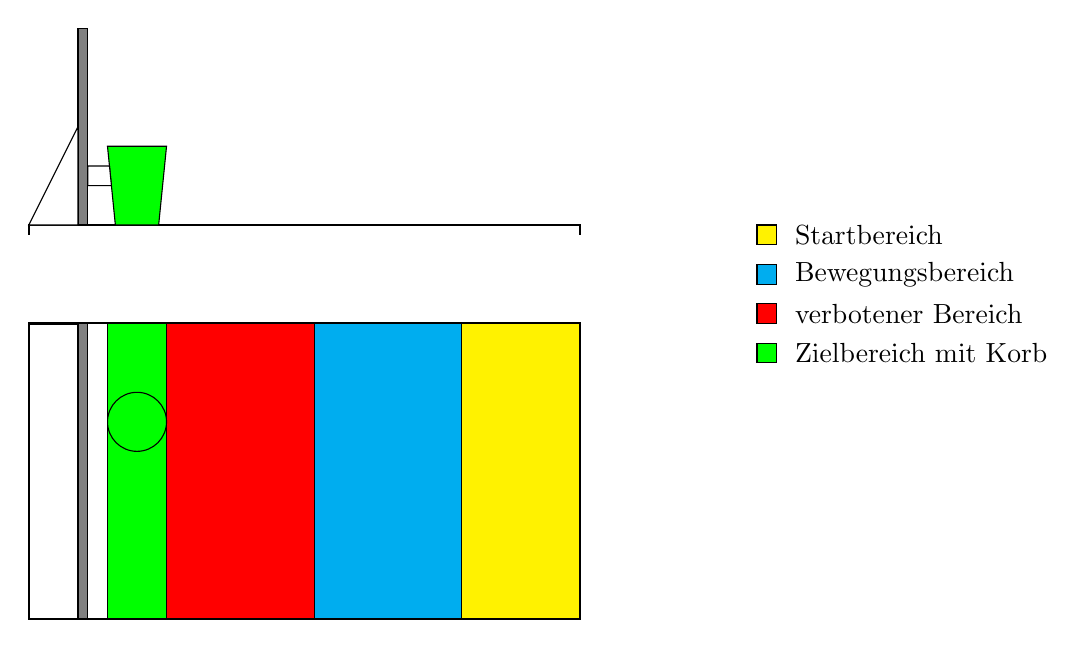
\begin{tikzpicture}[scale=0.025, rotate=90]
        \def \offset {200}          % Offset between Views of playfield
        \def \captionxoffset {130}  % Offset of caption in vertical distance
        \def \captionyoffset {-100} % Offset of caption in horizontal distance
        % playfield frame
        \draw[thick] (0,0) rectangle (150,280);
        \draw[thick] (\offset-5,0) -- (\offset,0) -- (\offset,280) -- (\offset-5,280);
        % startfield
        \draw[fill=yellow] (0,0) rectangle (150,60);
        % move field
        \draw[fill=cyan] (0,60) rectangle (150,135);
        % border line
        \draw[thick] (0,135) -- (150,135);
        % void field
        \draw[fill=red] (0,135) rectangle (150,210);
        % basket field
        \draw[fill=green] (0,210) rectangle (150,240);
        % basket
        \draw[fill=green] (100,225) circle [radius=15];
        \draw[fill=green] (\offset,214) -- (\offset+40,210) -- 
            (\offset+40,240) -- (\offset,236) -- (\offset,214);
        % gap filler
        \draw[fill=white] (0,240) rectangle (150,250);
        \draw[fill=white] (\offset+20,250) -- (\offset+20,238) -- (\offset+30,239) -- (\offset+30,250) -- (\offset+20,250);
        % wall
        \draw[fill=gray] (0,250) rectangle (150,255);
        \draw[fill=gray] (\offset,250) rectangle (\offset+100,255);
        \draw[fill=white] (\offset,255) -- (\offset+50,255) -- (\offset,280) -- (\offset,255);
        % caption
        \draw[fill=green]  (\captionxoffset+00,\captionyoffset) 
            rectangle node[right]{~ Zielbereich mit Korb}   
            (\captionxoffset+10,\captionyoffset+10);
        \draw[fill=red]    (\captionxoffset+20,\captionyoffset) 
            rectangle node[right]{~ verbotener Bereich}     
            (\captionxoffset+30,\captionyoffset+10);
        \draw[fill=cyan]   (\captionxoffset+40,\captionyoffset) 
            rectangle node[right]{~ Bewegungsbereich}       
            (\captionxoffset+50,\captionyoffset+10);
        \draw[fill=yellow] (\captionxoffset+60,\captionyoffset) 
            rectangle node[right]{~ Startbereich}           
            (\captionxoffset+70,\captionyoffset+10);
    \end{tikzpicture}
    \caption{Spielfeld}
    \label{fig:playfield}
\end{figure}

